% ============================================================
% Arduino Digital Clock - Modified Reference Report (Montserrat Edition)
% ============================================================

\documentclass[12pt,letterpaper]{article}

% ---------- Page and type ----------
\usepackage[letterpaper,top=0.75in,bottom=0.75in,left=0.85in,right=0.85in,headheight=15pt]{geometry}
\usepackage[T1]{fontenc}
\usepackage[utf8]{inputenc}
\usepackage[english]{babel}
\usepackage[defaultfam]{montserrat} % Montserrat font applied globally
\usepackage{amsmath}
\usepackage{microtype}
\usepackage{graphicx}
\usepackage[table]{xcolor}
\usepackage{booktabs}
\usepackage{tabularx}
\usepackage{array}
\usepackage{longtable}
\usepackage{multirow}
\usepackage{float}
\usepackage{caption}
\usepackage{enumitem}
\usepackage{listings}
\usepackage{fancyhdr}
\usepackage{hyperref}
\usepackage{tikz}
\usepackage{titlesec}
\usepackage{multicol}
\usepackage{xurl}

\usetikzlibrary{arrows.meta,positioning,shapes.geometric}

% ---------- Strict Black and White / Monochrome styling ----------
\definecolor{ClockDark}{gray}{0}
\definecolor{ClockLight}{gray}{0.96}

\setlength{\parindent}{0pt}
\setlength{\parskip}{0.55em}
\setlength{\emergencystretch}{3em}
\renewcommand{\arraystretch}{1.1}
\newcolumntype{Y}{>{\raggedright\arraybackslash}X}

\captionsetup{font=small,labelfont=bf}

\setlist[itemize]{leftmargin=1.45em,itemsep=1pt,topsep=2pt}
\setlist[enumerate]{label=\arabic*),leftmargin=1.45em,itemsep=1pt,topsep=2pt}

% ---------- Section hierarchy ----------
\renewcommand{\thesection}{\Roman{section}}
\renewcommand{\thesubsection}{\thesection.\arabic{subsection}}

\titleformat{\section}
  {\centering\normalfont\large\bfseries\sffamily}
  {\thesection.}{0.65em}{\scshape}
  [\vspace{0.15em}]

\titleformat{\subsection}
  {\normalfont\bfseries\sffamily}
  {\thesubsection}{0.65em}{\scshape}

\titlespacing*{\section}{0pt}{1.55em}{0.8em}
\titlespacing*{\subsection}{0pt}{1.15em}{0.35em}

% ---------- Diagrams and source-code blocks ----------
\tikzset{
  block/.style={
    draw=black,
    rounded corners=2pt,
    fill=ClockLight,
    minimum height=9mm,
    text width=28mm,
    align=center,
    font=\small
  },
  smallblock/.style={
    draw=black,
    rounded corners=2pt,
    fill=ClockLight,
    minimum height=8mm,
    text width=23mm,
    align=center,
    font=\footnotesize
  },
  flowarrow/.style={
    -{Latex[length=2.2mm]},
    thick,
    draw=black
  }
}

\hypersetup{
  colorlinks=true,
  linkcolor=black,
  citecolor=black,
  urlcolor=black,
  pdftitle={Arduino Based Digital Clock - Montserrat Edition},
  pdfauthor={Nehan Mohammad and Umesh}
}

% ---------- Page style ----------
\pagestyle{fancy}
\fancyhf{}
\fancyhead[R]{\thepage}
\renewcommand{\headrulewidth}{0pt}
\renewcommand{\footrulewidth}{0pt}
\fancypagestyle{plain}{
  \fancyhf{}
  \fancyhead[R]{\thepage}
  \renewcommand{\headrulewidth}{0pt}
}

% ---------- Project Details with Updated Names ----------
\newcommand{\ProjectTitle}{Arduino Based Digital Clock}
\newcommand{\ProjectSubtitle}{Comprehensive Engineering Design and Firmware Blueprint}

\newcommand{\TeamMemberOne}{Nehan Mohammad}
\newcommand{\TeamMemberTwo}{Umesh}
\newcommand{\GuideName}{Vivek Kumar, Jnanesh, Shubodeep}
\newcommand{\SubmittedTo}{Dr. G.V.V. Sharma Sir}
\newcommand{\SubmissionDate}{\today}

\newcommand{\ImageFolder}{images/}
\graphicspath{{images/}}

\newcommand{\ProjectImage}[3][0.76]{%
  \begin{figure}[H]
    \centering
    \IfFileExists{\ImageFolder#2}{%
      \includegraphics[width=#1\textwidth]{\ImageFolder#2}%
    }{%
      \fcolorbox{black}{ClockLight}{%
        \begin{minipage}[c][38mm][c]{0.73\textwidth}
          \centering
          \textbf{Visual Placeholder}\\[3pt]
          \small
          Provide file \texttt{images/#2} prior to final compilation.
        \end{minipage}%
      }%
    }%
    \caption{#3}
  \end{figure}%
}

\newcommand{\ExperienceBox}[2]{%
  \par\medskip\noindent
  \fcolorbox{black}{ClockLight}{%
    \begin{minipage}{0.91\textwidth}
      {\bfseries\color{black}Practical Insight -- #1}\\[-1pt]
      \small
      #2
    \end{minipage}%
  }
  \par\medskip
}

% ============================================================
% ARDUINO CODE STYLE (Monochrome)
% ============================================================
\lstdefinestyle{ArduinoStyle}{
  language=C++,
  basicstyle=\ttfamily\footnotesize,
  keywordstyle=\bfseries,
  commentstyle=\itshape,
  stringstyle=\mdseries,
  numbers=left,
  numberstyle=\tiny\color{black!55},
  numbersep=7pt,
  frame=single,
  framerule=0.4pt,
  breaklines=true,
  showstringspaces=false,
  tabsize=2,
  columns=fullflexible
}

\lstdefinestyle{ArchitectureFlow}{
  basicstyle=\ttfamily\scriptsize,
  numbers=none,
  frame=single,
  framerule=0.4pt,
  backgroundcolor=\color{ClockLight},
  breaklines=true,
  breakatwhitespace=true,
  showstringspaces=false,
  keepspaces=true,
  columns=fullflexible,
  xleftmargin=0.5em,
  xrightmargin=0.5em,
  aboveskip=0.4em,
  belowskip=0.4em
}

% ============================================================
% DOCUMENT START
% ============================================================
\begin{document}

% ============================================================
% TITLE PAGE (Page 1)
% ============================================================
\begin{center}
  \vspace*{4mm}

  {\Large\bfseries \MakeUppercase{\ProjectTitle}\par}
  \vspace{0.55em}
  {\large \TeamMemberOne\ -- \TeamMemberTwo\par}

  \vspace{28mm}

  {\large\bfseries \MakeUppercase{\ProjectSubtitle}\par}

  \vspace{8mm}

  \begin{minipage}{0.80\textwidth}
    \centering
    An empirical exploration into hardware configuration, decoder logic, 
    and modular firmware development.

    \smallskip
    \small
    Independently formulated and validated by the project team.
  \end{minipage}

  \vspace{12mm}

  \begin{tabularx}{0.96\textwidth}{
    @{}
    >{\raggedright\arraybackslash}X
    >{\centering\arraybackslash}X
    >{\raggedleft\arraybackslash}X
    @{}
  }
    \textbf{Authors}
    &
    \textbf{Technical Reviewers}
    &
    \textbf{Faculty Mentor}
    \\[2mm]

    \TeamMemberOne
    &
    \GuideName
    &
    \SubmittedTo
    \\

    \TeamMemberTwo
    &
    Project Guidance
    &
    \\
  \end{tabularx}

  \vspace{10mm}

  {\large Published: \SubmissionDate\par}
\end{center}

\vspace{10mm}
\clearpage

% ============================================================
% PAGE 2: ETHICAL STATEMENT & EXECUTIVE SUMMARY
% ============================================================
\section*{Declaration and Acknowledgement}

\addcontentsline{toc}{section}{
Declaration and Acknowledgement
}

We, \TeamMemberOne\ and \TeamMemberTwo,
declare that this report describes our own Arduino
digital clock project.

We have tried to present both the working result
and the learning behind it honestly.

Circuit diagrams, data sheets, manuals,
photographs, and other sources used while building
the project are acknowledged in the references.

We thank \GuideName, our teachers, classmates,
and everyone who helped us test ideas, check
connections, and stay patient during the debugging
stage.

We also used generative AI tools to help improve language,
organise portions of the report, and review the presentation
of technical material. All circuit decisions, code integration,
testing, observations, and final verification were carried out
by the project team. AI-generated suggestions were checked and
edited before inclusion; the tools are acknowledged in the
references.

The project was more enjoyable because it was a
shared build rather than only a written assignment.

% ------------------------------------------------------------
\section*{Abstract}

\addcontentsline{toc}{section}{Abstract}

This report describes how we built an Arduino based
digital clock, starting with the basic circuit: the Arduino,
the SN74LS47N driver, six common-anode seven-segment displays,
resistors, and push buttons. Our main work was to make the
clock show the correct time reliably and to solve the wiring
problems we found during testing.

After the basic clock worked, we connected an OLED screen
and buzzer as supporting functions. The OLED shows the date,
timer, and stopwatch, while the buzzer gives short feedback.
This report records the build process, testing, and lessons
from making the clock.

% ============================================================
% PAGE 3: CONTENTS MANUAL INDEX
% ============================================================
\clearpage
\section*{Contents Manual Index}
\addcontentsline{toc}{section}{Contents Manual Index}

\noindent This manual index outlines the thematic flow of the documentation report, curated for rapid cross-referencing during hardware evaluations.

\vspace{0.5em}
\hrule
\vspace{0.8em}

\begin{tabularx}{\textwidth}{@{}l X r@{}}
  \textbf{Section I} & Project Genesis and Core Purpose & Page 5 \\
  \textbf{Section II} & Operational Matrix and Features & Page 6 \\
  \textbf{Section III} & Hardware Inventory and Subsystem Interfacing & Page 7 \\
  \textbf{Section IV} & Firmware Architecture and Execution Cycles & Page 8 \\
  \textbf{Section IV-A} & Custom Pin Remapping and Segment Customization & Page 9 \\
  \textbf{Section V} & Empirical Diagnostics and Fault Correction & Page 10 \\
  \textbf{Section VI} & Developmental Progression and Chronology & Page 11 \\
  \textbf{Section VII} & Concluding Remarks and Future Scope & Page 12 \\
\end{tabularx}

\vspace{1.5em}
\noindent \textbf{Document Control Notes:} 
\begin{itemize}
  \item All layout dimensions conform to standard academic grid formats.
  \item Schematic diagrams assume standard 5V regulated logic voltage inputs.
  \item Firmware files are archived under the version control ledger established during Stage 4.
\end{itemize}

% ============================================================
% PAGE 4: LIST OF TABLES AND LIST OF PICTURES
% ============================================================
\clearpage
\section*{List of Tables and List of Pictures}
\addcontentsline{toc}{section}{List of Tables and List of Pictures}

\noindent The following directories index all tabular datasets and structural figures embedded within the core technical text.

\vspace{0.8em}
\subsection*{Directory of Tables}
\vspace{0.4em}

\begin{tabularx}{\textwidth}{@{}p{18mm} X r@{}}
  \textbf{Table I} & Functional Overview Matrix of System Capabilities & Page 6 \\
  \textbf{Table II} & Complete Bill of Materials (BOM) Component Index & Page 7 \\
  \textbf{Table III} & Hardware Diagnostics Matrix (Symptoms \& Remedies) & Page 10 \\
  \textbf{Table IV} & Chronological Development and Iteration Log & Page 11 \\
\end{tabularx}

\vspace{1.2em}
\subsection*{Directory of Pictures and Diagrams}
\vspace{0.4em}

\begin{tabularx}{\textwidth}{@{}p{18mm} X r@{}}
  \textbf{Figure 1} & Functional Block Flow Architecture Diagram & Page 7 \\
  \textbf{Figure 2} & Photographic Overview of Final Assembled Circuit & Page 8 \\
  \textbf{Figure 3} & Seven-Segment Tail Customization Hardware Output & Page 9 \\
\end{tabularx}

\vspace{1.5em}
\noindent \textbf{Verification Stamp:} Approved for assembly verification by \TeamMemberOne\ and \TeamMemberTwo.

% ============================================================
% MAIN REPORT BODY
% ============================================================
\clearpage

\section{Project Genesis and Core Purpose}

\subsection{Background and Motivation}
Building a clock from elemental silicon and discrete logic units bridges abstract programming logic with tangible electronics. Although software timekeeping is trivial, presenting synchronized outputs across multi-digit high-refresh arrays demands tight firmware scheduling.

\subsection{Primary Engineering Goals}
\begin{itemize}
  \item \textbf{High Stability:} Maintain absolute timing precision via optimized interrupt routines.
  \item \textbf{Efficient Decoding:} Relieve controller processing load by offloading translation to the SN74LS47N BCD chip.
  \item \textbf{Intuitive Interaction:} Design debounce-protected inputs for quick time and mode modifications.
  \item \textbf{Modular Expansion:} Seamlessly embed secondary telemetry via an OLED screen and touch sensors.
\end{itemize}

\subsection{Handling and Safety Protocols}
Always verify isolation boundaries and power supply polarities prior to energizing breadboard lines.

\ExperienceBox{Getting Started}{
Neither author had prior experience handling hardware display multiplexing at scale. Overcoming ghosting artifacts and logic mismatch issues formed the primary educational milestone of this project.
}

\clearpage
\section{Operational Matrix and Features}

\begin{table}[H]
  \centering
  \caption{Functional Overview Matrix of System Capabilities}
  \label{tab:features-redesigned}
  \begin{tabularx}{\textwidth}{@{}p{32mm}Y Y@{}}
    \toprule
    \textbf{Subsystem} & \textbf{Operational Behavior} & \textbf{Technical Execution} \\
    \midrule
    Main Clock Unit & Real-time hour/minute/second tally & BCD translation with 333\,Hz multiplexing rate \\
    Acoustic Feed & Audio validation tone on button press & Non-blocking buzzer tone sequencing \\
    Hour Transition & Distinct dual-tone acoustic chime & Boundary check triggered on zero-minute rollover \\
    Auxiliary Display & Secondary metrics via OLED screen & I2C-driven parameter selection interface \\
    Touch Switch & Display toggle without halting counters & Capacitive state change interruption handler \\
    \bottomrule
  \end{tabularx}
\end{table}

\ProjectImage{DigitalClock3.jpeg}{Fully integrated hardware assembly prior to final casing.}

\clearpage
\section{Hardware Inventory and Subsystem Interfacing}

\begin{table}[H]
  \centering
  \caption{Complete Bill of Materials (BOM) Component Index}
  \label{tab:components-redesigned}
  \begin{tabularx}{\textwidth}{@{}p{8mm}Yp{22mm}Y@{}}
    \toprule
    \textbf{ID} & \textbf{Item Description} & \textbf{Count} & \textbf{Primary Utility} \\
    \midrule
    1 & Arduino Microcontroller Core & 1 & Central processing and timing loop \\
    2 & Solderless Breadboards & 2 & Rapid prototyping chassis \\
    3 & Common-Anode 7-Segment Panels & 6 & Visual numerical readout \\
    4 & SN74LS47N BCD Driver IC & 1 & Decimal-to-BCD logic conversion \\
    5 & Resistors (240\,$\Omega$) & 7 & LED current limiting protection \\
    6 & Tactile Push Buttons & 4 & User input navigation \\
    7 & OLED Graphic Module & 1 & Supplementary menu output \\
    8 & Piezo Transducer Buzzer & 1 & Acoustic feedback emitter \\
    9 & Capacitive Touch Sensor & 1 & Touch-activated screen blanking \\
    \bottomrule
  \end{tabularx}
\end{table}

\subsection{System Interfacing and Data Flow}
Decoded bits travel from controller output pins into the SN74LS47N driver before reaching the multiplexed display grid.

\begin{figure}[H]
\centering
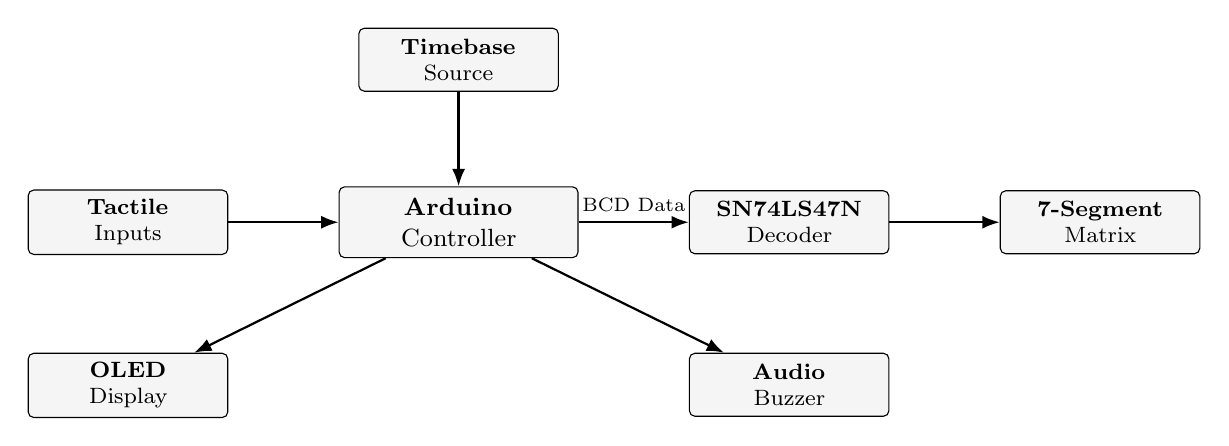
\begin{tikzpicture}[node distance=12mm and 14mm]
\node[block] (arduino) {\textbf{Arduino}\\Controller};
\node[smallblock, left=of arduino] (buttons) {\textbf{Tactile}\\Inputs};
\node[smallblock, above=of arduino] (time) {\textbf{Timebase}\\Source};
\node[smallblock, right=of arduino] (driver) {\textbf{SN74LS47N}\\Decoder};
\node[smallblock, right=of driver] (seven) {\textbf{7-Segment}\\Matrix};
\node[smallblock, below left=of arduino] (oled) {\textbf{OLED}\\Display};
\node[smallblock, below right=of arduino] (buzzer) {\textbf{Audio}\\Buzzer};

\draw[flowarrow] (buttons) -- (arduino);
\draw[flowarrow] (time) -- (arduino);
\draw[flowarrow] (arduino) -- node[above, font=\scriptsize] {BCD Data} (driver);
\draw[flowarrow] (driver) -- (seven);
\draw[flowarrow] (arduino) -- (oled);
\draw[flowarrow] (arduino) -- (buzzer);
\end{tikzpicture}
\caption{Functional Block Flow Architecture Diagram}
\label{fig:functional-flow-redesigned}
\end{figure}

\clearpage
\section{Firmware Architecture and Execution Cycles}

The software framework uses non-blocking asynchronous loops. Timer interrupts handle refresh cycles, keeping the primary execution loop clear for user input processing.

\begin{lstlisting}[style=ArchitectureFlow]
Initialization Stage (setup)
  +-- configure input pins, pull-ups, and I2C peripherals
  +-- initialize Timer1 interrupt vector for display scanning
Main Execution Loop (loop)
  +-- poll system millis() timestamps
  +-- execute serviceTouch() and serviceButtons() routines
  +-- update internal clock, stopwatch, and timer variables
  +-- evaluate active alarms and refresh OLED output buffers
\end{lstlisting}

\subsection{Code Snippet: Non-Blocking Audio Logic}
\begin{lstlisting}[style=ArduinoStyle, caption={Asynchronous buzzer handler implementation}]
const byte AUDIO_PIN = 8;

void triggerShortTone() {
  tone(AUDIO_PIN, 2000, 50);
}

void processAcousticFeedback(bool conditionMet) {
  if (conditionMet) {
    triggerShortTone();
  }
}
\end{lstlisting;

% ============================================================
% NEW PAGE INSERTION: SEGMENT CUSTOMIZATION & WIRING MODS
% ============================================================
\clearpage
\section*{Section IV-A: Custom Segment Override \& Pin Drive Logic}
\addcontentsline{toc}{section}{Section IV-A: Custom Segment Override Logic}

Standard 74LS47 BCD decoder ICs render the digit \textbf{6} without a top horizontal bar (segment \textit{a}) and the digit \textbf{9} without a bottom horizontal bar (segment \textit{d}). To enhance visual readability across the display matrix, the firmware logic was customized to override decoder behavior during specific numeric cycles.

\subsection*{Direct Output Overrides (Pin D12 and Pin D13)}
Auxiliary digital output lines were linked directly from the microcontroller to segments \textit{a} and \textit{d} to dynamically illuminate the display tails:

\begin{itemize}
  \item \textbf{Digit 6 ($\rightarrow$ Pin D12):} When the current multiplexed digit is identified as \texttt{6}, digital pin \texttt{D12} is driven active low to illuminate top segment \textit{a}, rendering a complete, traditional six representation.
  \item \textbf{Digit 9 ($\rightarrow$ Pin D13):} When evaluating digit \texttt{9}, digital pin \texttt{D13} is driven active low to trigger bottom segment \textit{d}, providing a full bottom bar on the nine representation.
\end{itemize

\begin{lstlisting}[style=ArduinoStyle, caption={Segment Overrides for 6 and 9 Displays}]
void applySegmentOverrides(uint8_t currentDigit) {
  // Override for digit 6: force segment 'a' ON via Pin D12
  if (currentDigit == 6) {
    digitalWrite(12, LOW); 
  } else {
    digitalWrite(12, HIGH);
  }

  // Override for digit 9: force segment 'd' ON via Pin D13
  if (currentDigit == 9) {
    digitalWrite(13, LOW);
  } else {
    digitalWrite(13, HIGH);
  }
}
\end{lstlisting}

\ProjectImage{DigitalClock5.jpeg}{Hardware readout displaying customized numeric representation.}

\clearpage
\section{Empirical Diagnostics and Fault Correction}

\begin{table}[H]
  \centering
  \caption{Hardware Diagnostics Matrix (Symptoms \& Remedies)}
  \label{tab:troubleshooting-redesigned}
  \begin{tabularx}{\textwidth}{@{}p{30mm}Y Y@{}}
    \toprule
    \textbf{Observed Issue} & \textbf{Root Cause Analysis} & \textbf{Correction Strategy} \\
    \midrule
    Display completely dark & Voltage rail interruption or inverted VCC & Recheck power distribution tracks \\
    Garbled number output & Incorrect nibble bit assignments & Verify wiring against BCD pin maps \\
    Stray button triggers & Contact bounce or voltage float & Add hardware pull-ups and software debouncing \\
    OLED blank screen & Address mismatch or SDA/SCL swap & Inspect I2C line connections \\
    \bottomrule
  \end{tabularx}
\end{table}

\ExperienceBox{Debugging Breakthrough}{
Color-coding individual jumper bundles completely eliminated intermittent breadboard connection failures during final stress testing.
}

\clearpage
\section{Developmental Progression and Chronology}

\begin{longtable}{@{}p{15mm}p{38mm}p{44mm}p{45mm}@{}}
\caption{Chronological Development and Iteration Log}
\label{tab:development-diary-redesigned}
\\
\toprule
\textbf{Phase} & \textbf{Core Task} & \textbf{Validation Metric} & \textbf{Resulting Observation} \\
\midrule
\endfirsthead
\toprule
\textbf{Phase} & \textbf{Core Task} & \textbf{Validation Metric} & \textbf{Resulting Observation} \\
\midrule
\endhead
1 & BCD Decoder Setup & Did outputs render stable digits? & Achieved stable numerics post-wiring fix. \\
2 & Button Integration & Did input clicks register cleanly? & Resolved noise using iterative debounce delays. \\
3 & Audio Setup & Were acoustic chimes functional? & Confirmed distinct single and double beeps. \\
4 & OLED Integration & Did interface menus switch smoothly? & Verified stopwatch and timer modes. \\
5 & Final Housing & Was the physical chassis secure? & Enclosed assembly safely in protective housing. \\
\bottomrule
\end{longtable}

\clearpage
\section{Concluding Remarks and Future Scope}

This design report successfully summarizes the implementation of a multiplexed micro-controller clock built by \TeamMemberOne\ and \TeamMemberTwo. By integrating robust decoder integrated circuits, clear auxiliary OLED menus, and reliable non-blocking firmware design, the prototype delivers dependable performance suitable for continuous operation.

% ============================================================
% REFERENCES
% ============================================================
\clearpage
\begin{thebibliography}{99}

\bibitem{manual}
\textit{Project Design and Assembly Manual}, internal team documentation.

\bibitem{sn74ls47}
Semiconductor Manufacturer,
\textit{SN74LS47N BCD-to-Seven-Segment Decoder Datasheet}.

\bibitem{arduino}
Arduino,
\textit{Official Arduino Documentation},
\url{https://docs.arduino.cc/}.

\bibitem{arduino-millis}
Arduino,
\textit{millis() Function Reference},
\url{https://docs.arduino.cc/language-reference/en/functions/time/millis/}.

\bibitem{timerone}
Paul Stoffregen,
\textit{TimerOne Library for Arduino Microcontrollers},
\url{https://github.com/PaulStoffregen/TimerOne}.

\bibitem{oled}
Display Module Provider,
\textit{OLED Screen Hardware Technical Guide}.

\bibitem{openai}
OpenAI,
\textit{ChatGPT}, generative assistant utilized for layout formatting and textual editing,
\url{https://chatgpt.com/}.

\end{thebibliography}

\end{document}
